\documentclass{article}
\usepackage[utf8]{inputenc}
\usepackage{cancel}
\usepackage{amsthm,amssymb,amsmath}
\usepackage{mathtools}
\usepackage{tikz}
\usetikzlibrary{calc}
\usetikzlibrary{positioning}
\usepackage{parskip}
\usepackage{float}
\newtheorem{theorem}{Theorem}[section]
\newtheorem{corollary}{Corollary}[theorem]
\newtheorem{lemma}[theorem]{Lemma}
\setlength{\parskip}{1em}
\newcommand{\NN}{\mathbb{N}}
\newcommand{\ZZ}{\mathbb{Z}}
\newcommand{\RR}{\mathbb{R}}
\newcommand{\QQ}{\mathbb{Q}}
\newcommand{\CC}{\mathbb{C}}

\title{MAT 4800 Homework \# 3}
\author{Noah Reef }
\date{Spring 2023}

\usepackage{natbib}
\usepackage{graphicx}

\begin{document}
\maketitle
\section*{Problem \#1}
\subsection*{Part a}
Suppose we are given the following matrix,

\begin{equation*}
   A = \begin{pmatrix}
    1 & 0 & 0 \\
    0 & 3 & 0 \\
    0 & 0 & 5
    \end{pmatrix}
\end{equation*}
whose corresponding characteristic polynomial is,
\begin{equation*}
    (1-\lambda)(3-\lambda)(5-\lambda) = 0
\end{equation*}
which implies $\lambda = 1,3,5 > 0$. Thus by \textit{Theorem 1.5.1}, then $A$ is \textbf{Positive Definite}.

\subsection*{Part b}
Suppose we are given the following matrix,

\begin{equation*}
   A = \begin{pmatrix*}[r]
    -1 & 0 & 0 \\
    0 & -3 & 0 \\
    0 & 0 & -2
    \end{pmatrix*}
\end{equation*}
whose corresponding characteristic polynomial is,
\begin{equation*}
    (-1-\lambda)(-3-\lambda)(-2-\lambda) = 0
\end{equation*}
which implies $\lambda = -1,-3,-2 < 0$. Thus by \textit{Theorem 1.5.1}, then $A$ is \textbf{Negative Definite}.

\subsection*{Part c}
Suppose we are given the following matrix,

\begin{equation*}
   A = \begin{pmatrix*}[r]
    7 & 0 & 0 \\
    0 & -8 & 0 \\
    0 & 0 & 5
    \end{pmatrix*}
\end{equation*}
whose corresponding characteristic polynomial is,
\begin{equation*}
    (7-\lambda)(-8-\lambda)(5-\lambda) = 0
\end{equation*}
which implies $\lambda = 7,-8,5$. Thus by \textit{Theorem 1.5.1}, then $A$ is \textbf{Indefinite}.

\subsection*{Part d}
Suppose we are given the following matrix,

\begin{equation*}
   A = \begin{pmatrix}
    3 & 1 & 2 \\
    1 & 5 & 3 \\
    2 & 3 & 7
    \end{pmatrix}
\end{equation*}
whose principal minors are
\begin{align*}
    \Delta_1 &= 3 > 0\\
    \Delta_2 &= 15-1 = 14 > 0 \\
    \Delta_3 &= 3(35-9) - (7-6) + 2(3-10) = 63 > 0
\end{align*}
since $\Delta_1, \Detal_2, \Delta_3 > 0$. Thus by \textit{Theorem 1.3.3}, then $A$ is \textbf{Definite Positive}.

\subsection*{Part e}
Suppose we are given the following matrix,

\begin{equation*}
   A = \begin{pmatrix*}[r]
    -4 & 0 & 1 \\
    0 & -3 & 2 \\
    1 & 2 & -5
    \end{pmatrix*}
\end{equation*}
whose principal minors are
\begin{align*}
    \Delta_1 &= -4 < 0\\
    \Delta_2 &= 12 > 0 \\
    \Delta_3 &= -4(15-4) + (0 - (-3)) = -41 < 0
\end{align*}
since $(-1)^k\Delta_k > 0$. Thus by \textit{Theorem 1.3.3}, then $A$ is \textbf{Definite Negative}.

\section*{Problem \#2}
\subsection*{Part a}
Suppose we are given the following matrix,

\begin{equation*}
   A = \begin{pmatrix*}[r]
    -1 & 2 \\
    2 & 3 
    \end{pmatrix*}
\end{equation*}

Then
\begin{equation*}
    Q_A(\vec{x}) = x_1(-x_1 + 2x_2) + x_2(2x_1 + 3x_2) = -x_1^2 + 4x_1x_2 + 3x_2^2 
\end{equation*}

\subsection*{Part b}
Suppose we are given the following matrix,

\begin{equation*}
   A = \begin{pmatrix*}[r]
    2 & -3 \\
    -3 & 0 
    \end{pmatrix*}
\end{equation*}

Then
\begin{equation*}
    Q_A(\vec{x}) = x_1(2x_1 - 3x_2) + x_2(-3x_1) = 2x_1^2 -6x_1x_2
\end{equation*}

\subsection*{Part c}
Suppose we are given the following matrix,

\begin{equation*}
   A = \begin{pmatrix*}[r]
    1 & -1 & 0\\
    -1 & -2 & 2 \\
    0 & 2 & 3
    \end{pmatrix*}
\end{equation*}

Then
\begin{equation*}
    Q_A(\vec{x}) = x_1(x_1 - x_2) + x_2(-x_1-2x_2 + 2x_3) + x_3(2x_2 + 3x_3) 
\end{equation*}

\section*{Problem \#3}
\subsection*{Part a}
Suppose we are given the quadratic form of 
\begin{equation*}
    Q_A(\vec{x}) = 3x_1^2 - x_1x_2 + 2x_2^2
\end{equation*}

results from the matrix 
\begin{equation*}
    A = \begin{pmatrix*}[r]
        3 & 0  \\
         -1 & 2 
    \end{pmatrix*}
\end{equation*}

thus,

\subsection*{Part b}
Suppose we are given the quadratic form of 
\begin{equation*}
    Q_A(\vec{x}) = x_1^2 + 2x_2^2 - 3x_3^2 + 2x_1x_2 - 4x_1x_3 + 6x_2x_3
\end{equation*}
results from the matrix 
\begin{equation*}
    A = \begin{pmatrix*}[r]
        1 & 0 & 0 \\
        2 & 2 & 6\\
        -4&0 & -3
    \end{pmatrix*}
\end{equation*}
\subsection*{Part c}
Suppose we are given the quadratic form of 
\begin{equation*}
    Q_A(\vec{x}) = 2x_1^2 - 4x_3^2 + x_1x_2 - x_2x_3
\end{equation*}
results from the matrix 
\begin{equation*}
    A = \begin{pmatrix*}[r]
        2 & 1 & 0\\
       0 & 0 & -1\\
       0 &0  & -4
    \end{pmatrix*}
\end{equation*}

\section*{Problem \#4}
Suppose that $f(\vec{x})$ is defined on $\RR^3$ by
\begin{equation*}
    f(\vec{x}) = c_1x_1^2 + c_2x_2^2 + c_3x_3^2 + c_4x_1x_2 + c_5x_1x_3 + c_6x_2x_3
\end{equation*}
to show that the Quadratic Form of $f(\vec{x})$ is associated with $\frac{1}{2}Hf$, we first compute $\nabla f(\vec{x})$,

\begin{equation*}
    \nabla f(\vec{x}) = \begin{bmatrix*}
        2c_1x_1 +c_4x_2 + c_5x_3 \\
        2c_2x_2 + c_4x_1 + c_6x_3 \\
        2c_3x_3 + c_5x_1 + c_6x_2
    \end{bmatrix*}
\end{equation*}

then we compute the Hessian as

\begin{equation*}
    Hf = \begin{bmatrix*}
        2c_1 & c_4 & c_5 \\
        c_4 & 2c_2 & c_6 \\
        c_5 & c_6 & 2c_3
    \end{bmatrix*}
\end{equation*}
\begin{equation*}
 \frac{1}{2} Hf = \begin{bmatrix*}
        c_1 & \frac{1}{2}c_4 & \frac{1}{2}c_5 \\
        \frac{1}{2}c_4 & c_2 & \frac{1}{2}c_6 \\
        \frac{1}{2}c_5 & \frac{1}{2}c_6 & c_3
    \end{bmatrix*}
\end{equation*}
Then computing the quadratic form,
\begin{align*}
    Q_{\frac{1}{2}Hf}(\vec{x}) &= x_1(c_1x_1 + \frac{1}{2}c_4x_2 + \frac{1}{2}c_5x_3) + x_2(\frac{1}{2}c_4x_1 + c_2x_2 +  \frac{1}{2}c_6x_3) + x_3(\frac{1}{2}c_5x_1 + \frac{1}{2}c_6x_2 + c_3x_3) \\
    &= c_1x_1^2 + c_2x_2^2 + c_3x_3^2 + c_4x_1x_2 + c_5x_1x_3 + c_6x_2x_3
\end{align*}

Expanding out the Quadratic form for $\RR^4$, we have
\begin{equation*}
     f(\vec{x}) = c_1x_1^2 + c_2x_2^2 + c_3x_3^2 + c_4x_4^2 + c_5x_1x_2 + c_6x_1x_3 + c_7x_2x_3 + c_8x_1x_4 + c_9x_2x_4 + c_{10}x_3x_4
\end{equation*}

giving us,

\begin{equation*}
    \nabla f(\vec{x}) = \begin{bmatrix*}
        2c_1x_1 +c_5x_2 + c_6x_3 + c_8x_4 \\
        2c_2x_2 + c_5x_1 + c_7x_3 + c_9x_4\\
        2c_3x_3 + c_6x_1 + c_7x_2 + c_{10}x_4 \\
        2c_4x_4 + c_8x_1 + c_9x_2 + c_{10}x_3
    \end{bmatrix*}
\end{equation*}

\begin{equation*}
    Hf = \begin{bmatrix*}
        2c_1 & c_5 & c_6 & c_8\\
        c_5 & 2c_2 & c_7 & c_9\\
        c_6 & c_7 & 2c_3 & c_{10}\\
        c_8 & c_9 & c_{10} & 2c_4
    \end{bmatrix*}
\end{equation*}

\begin{equation*}
     \frac{1}{2}Hf = \begin{bmatrix*}
        c_1 & \frac{1}{2}c_5 & \frac{1}{2}c_6 & \frac{1}{2}c_8\\
        \frac{1}{2}c_5 & c_2 & \frac{1}{2}c_7 & \frac{1}{2}c_9\\
        \frac{1}{2}c_6 & \frac{1}{2}c_7 & c_3 & \frac{1}{2}c_{10}\\
        \frac{1}{2}c_8 & \frac{1}{2}c_9 & \frac{1}{2}c_{10} & c_4
    \end{bmatrix*}
\end{equation*}
and,
\begin{equation*}
    Q_{\frac{1}{2}Hf}(\vec{x}) =c_1x_1^2 + c_2x_2^2 + c_3x_3^2 + c_4x_4^2 + c_5x_1x_2 + c_6x_1x_3 + c_7x_2x_3 + c_8x_1x_4 + c_9x_2x_4 + c_{10}x_3x_4
\end{equation*}

\section*{Problem \#5}
Suppose you are given the following,

\begin{equation*}
    f(x_1,x_2,x_3) = 3x_1^2 + 2x_2^2 + 2x_3^2+2x_1x_2 + 2x_2x_3 + 2x_1x_3
\end{equation*}

First we can compute $\nabla f(x_1,x_2,x_3) $,

\begin{equation*}
    \nabla f(x_1,x_2,x_3) = \begin{bmatrix*}
        6x_1 + 2x_2 + 2x_3\\
        4x_2 + 2x_1 + 2x_3\\
        4x_3 + 2x_2 + 2x_1
    \end{bmatrix*}
\end{equation*}

then we compute the Hessian,

\begin{equation*}
    Hf = \begin{bmatrix*}
        6 & 2 & 2 \\
        2 & 4& 2\\
        2 & 2 & 4
    \end{bmatrix*}
\end{equation*}

Now that we have computed the Hessian, now we compute the Principle Minors as
\begin{align*}
    \Delta_1 &= 6 > 0\\
    \Delta_2 &= 24 - 4 = 20 > 0 \\
    \Delta_3 &= 56 > 0
\end{align*}

Thus the Hessian is \textbf{Positive Definite} and thus the critical points are \textit{Strict Global Minimizers}

\section*{Problem \#6}
Suppose we are given the following function,

\begin{equation*}
    f(x_1,x_2) = x_1^5 - x_1x_2^6
\end{equation*}
we first compute $\nabla f(x_1,x_2)$ to get,
\begin{equation*}
    \nabla f(x_1,x_2) = \begin{bmatrix*}[r]
        5x_1^4 - x_2^6\\
        -6x_1x_2^5
    \end{bmatrix*}
\end{equation*}

which we see by plugging in $(0,0)$ we get $\nabla f(0,0) = 0$, thus $(0,0)$ is a critical point of $f(x_1,x_2)$. But we see that

\begin{align*}
    f(x_1,0) = x_1^5
\end{align*}

which is positive for $x_1 > 0$, negative for $x_1 < 0$, and $0$ at $x_1 = 0$, thus $(0,0)$ is neither a minimum or maximum.


\section*{Problem \#7}

\subsection*{Part a}
Suppose we are given the following function,

\begin{equation*}
    f(x_1,x_2) = x_1^3 - 3ax_1x_2 + x_2^3
\end{equation*}

Here we see that,

\begin{equation*}
    \lim_{x_1 \to \infty}f(x_1,0) = +\infty
\end{equation*}
Tells us that $f(x_1,x_2)$ has no global maximimizers.
\subsection*{Part b}
We see that by computing the gradient as,

\begin{equation*}
    \nabla f(x_1,x_2) = \begin{bmatrix*}[r]
        3x_1^2-3ax_2 \\
        -3ax_1 + 3x_2^2
    \end{bmatrix*}
\end{equation*}

and,

\begin{equation*}
    Hf = \begin{bmatrix*}[r]
        6x_1 & -3a \\
        -3a & 6x_2
    \end{bmatrix*}
\end{equation*}

to find the critical points of $f$ we compute,
\begin{align*}
    3x_1^2-3ax_2 &= 0 \\
    -3ax_1 + 3x_2^2 &= 0
\end{align*}

Solving the above system we see that the two critical points are $(0,0)$ and $(a,a)$.

Here we see that,
\begin{equation*}
    Hf(0,0) = \begin{bmatrix*}[r]
        0 & -3a \\
        -3a & 0
    \end{bmatrix*}
\end{equation*}

here we compute the eigenvalues as, $\lambda = \pm 3a$ thus $Hf(0,0)$ is indefinite and hence $(0,0)$ is a saddle for all $a \neq 0$, by \textit{Theorem 1.3.7}. Then for $(a,a)$ we get,

\begin{equation*}
    Hf(a,a) = \begin{bmatrix*}[r]
        6a & -3a \\
        -3a & 6a
    \end{bmatrix*}
\end{equation*}

which we see that,

\begin{align*}
    \Delta_1 &= 6a \\
    \Delta_2 &= 27a^2
\end{align*}

If $a > 0$, then $Hf(a,a)$ is Positive Definite and $(a,a)$ is a local minimum. If $a < 0$, then $Hf(a,a)$ is Negative Definite and $(a,a)$ is a local maximum.

\section*{Problem \#8}

\begin{figure}[H]
    \centering
    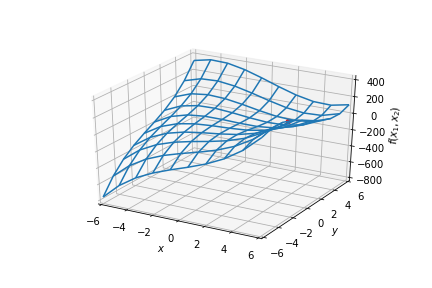
\includegraphics[scale=0.6]{aPos.png}
    \caption{Plot of $f(x,y)$ when $a = 3$}
    \label{fig:my_label}
\end{figure}

\begin{figure}[H]
    \centering
    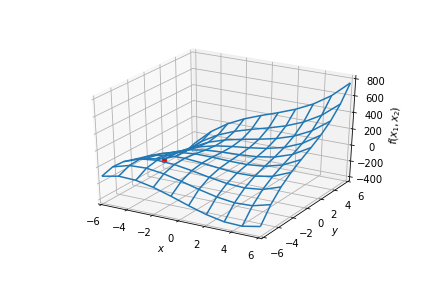
\includegraphics[scale=0.6]{aNeg.png}
    \caption{Plot of $f(x,y)$ when $a = -3$}
    \label{fig:my_label}
\end{figure}

\section*{Problem \#9}
Suppose we are given,
\begin{equation*}
    f(x,y) = x^3 + e^{3y} - 3xe^y
\end{equation*}

and compute the gradient as,

\begin{equation*}
    \nabla f(x,y) = \begin{bmatrix*}[r]
        3x^2 - 3e^y \\
        3e^{3y} - 3xe^y
    \end{bmatrix*}
\end{equation*}

to find the critical points, we compute the following

\begin{align*}
    3x^2 - 3e^y &= 0\\
        3e^{3y} - 3xe^y &= 0
\end{align*}

solving the system above we get the critical point to be $(1,0)$. Next we compute the Hessian as,

\begin{equation*}
    Hf = \begin{bmatrix*}[r]
        6x & -3e^y \\
        -3e^y & 9e^{3y}-3xe^y
    \end{bmatrix*}
\end{equation*}
and computing,
\begin{equation*}
    Hf(1,0) = \begin{bmatrix*}[r]
        6 & -3 \\
        -3 & 6
    \end{bmatrix*}
\end{equation*}
and see that $Hf(1,0)$ is positive definite since $\Delta_1 = 6 > 0, \Delta_2 = 27 >0$, thus $(1,0)$ is a local minimizer. However since,

\begin{equation*}
    \lim_{x_1 \to -\infty}f(x_1,0) = -\infty
\end{equation*}

We see that $f(x,y)$ has no global minimizers, thus $(1,0)$ cannot be a global minimizer.
\section*{Problem \#10}

\begin{figure}[H]
    \centering
    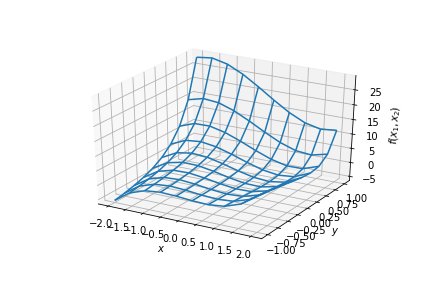
\includegraphics[scale=0.6]{graph3.png}
    \caption{Plot of $f(x,y) =  x^3 + e^{3y} - 3xe^y$}
    \label{fig:my_label}
\end{figure}

\begin{figure}[H]
    \centering
    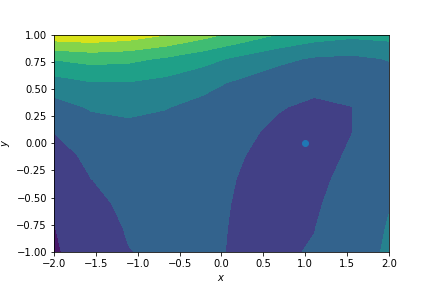
\includegraphics[scale=0.6]{graph3Contour.png}
    \caption{Contour Plot of $f(x,y) =  x^3 + e^{3y} - 3xe^y$}
    \label{fig:my_label}
\end{figure}

\end{document}